\chapter{The tokenized approach}\label{chap:approach}

In the example from the beginning, the problem was that both agents $a$ and $b$ wanted to pull the lever to their own goal which results in infinite executions. This problem can be eliminated by introducing a token. With a token, only the player that has the token gets to execute an action. If the agent is done with their own actions, then they can pass the token on to the next player.

The easiest way to introduce the token is seemingly random. Some undefined agent has the token in the beginning. The advantage is that you do not have to define anything in the beginning, but this is also a disadvantage, since this token is defined, but the agent that has it in the beginning is not. Here, giving the token to the next player would have to be added to the set of actions.

There are three other ways to introduce a token to this game. \todo{Du nimmst bisher keine Referenz zum Kapitel davor. Wuerde das bedeuten, dass man das "Token nehmen" und "Token abgeben" als Aktion in den Planungsalgorithmus einfuehren muss. Dann wuerde ich das hier schreiben.}
\begin{enumerate}
  \item ``Table token'' - the token is lying on a table and one of the agents can take the token in the beginning. \\
  The disadvantage is that maybe no agent would take the token.
  \item ``give token'' - in the specification of the game it is also specified which agent will have the token in the beginning. \\
  The problem with this introduction is that in every new game, this has to be written in the definition of the game. In order for the game to be efficient, it should be given to a player who has found a plan.
  \item ``random token'' - the token is given to a random agent in the beginning. If that agent can not preform any action it can pass the token to a player who can. \\
  One disadvantage would be that an agent who knows nothing and has no action will prevent the game from ever reaching a goal state.
\end{enumerate}



\section{Infinite executions to finite executions}

We are now going to describe a function that takes a regular planning task and tokenize that task. The goal with the tokens is that only one player gets to make a move at a time.

Given a regular planning task $\Pi = \langle s_0, A, \omega, \gamma \rangle $, the function \textit{tokenize} will transform the regular planning task into a tokenized planning task so that for all $a \in A$:
 if $a = \langle pre, \textit{eff} \rangle$, then
   $tokenize(a) =\langle pre \wedge hasToken^{\omega(a)}, \textit{eff} \rangle$. \\
Further we define an action
    $ giveToken^{ij} = \langle hasToken^i, \neg hasToken^i \wedge hasToken^j \rangle $
    for all $i,j \in \mathcal{A}$ with $i \not = j$. \\
Then $ A^{Token}=\{tokenize(a)|a \in A\} \cup \{giveToken^{ij}|i,j \in \mathcal{A}, i \not = j\}$. \\
Moreover: $\omega^{Token}(tokenize(a))= \omega(a)$ for all $a \in A$,
and $\omega^{Token}(giveToken^{ij}) = i$ for all $i,j \in \mathcal{A}$. \\
$s_0^{Token} = s_0 \cup \{\neg hasToken^i|i \in \mathcal{A} \backslash j\} \cup hasToken^j$ \\
With $j$ depending on the way the token should be introduced to the token:
\begin{enumerate}
  \item Table Token:
    The first agent to take the token off the table.
  \item give Token:
    a specified agent to be determined by the game maker
  \item random Token:
    a random agent
\end{enumerate}



Then $ \Pi^{\text{Token}} = \langle s_0, A ^{\text{Token}}, \omega ^{\text{Token}}, \gamma \rangle $.

The action $giveToken$ can have different costs in this case. In searching for the optimal plan the search tree can have a smaller width, but therefore will probably have a deeper depth. This could be researched in the future. \todo{Wie?}

\extend{überleitender Satz}

\begin{theorem}
Under the condition of optimal plans one can prevent the appearance of infinite executions in solvable games with asynchronous execution order with the introduction of a token based execution order.
\end{theorem}

\begin{proof}[proof sketch]
  The game is finished when the agent that has the token reaches a goal state. When an agent that has a plan gets handed the token, that player has two possible actions:
  \begin{enumerate}
    \item keep the token and execute an action, which will lower the subjective costs of the remaining policy profile or
    \item give the token to the next player. in order to pass on the token the player that has found the plan would have already performed a perspective shift for the next player, in order to check if the next player could also find that plan and calculated the subjective cost of the remaining plan. The player that receives the token will always execute that plan or find a better plan and execute the better plan.
  \end{enumerate}
  Every agent that will get the token in the plan will decrease the subjective cost of the policy profile, and because every agent decreases the subjective cost, the game is executable in infinite executions.
\end{proof}

\section{The prevention of deadlocks}

A deadlock for a policy profile $(\pi_i)_{i \in \mathcal{A}}$ is a global state such that:
\begin{enumerate}
  \item $s$ is not a goal state \\
    Something still needs to be done
  \item $s \in \text{Dom}(\pi_i)$ for some $i \in \mathcal{A}$ \\
    Someone wants something to be done
  \item $\omega(a) \neq i$ for all $i \in \mathcal{A}$ and $a \in \pi_i(s)$ \\
    Nothing will be done because of incompatible individual policies
\end{enumerate}

\begin{wrapfigure}{l}{0.2\linewidth}
\centering
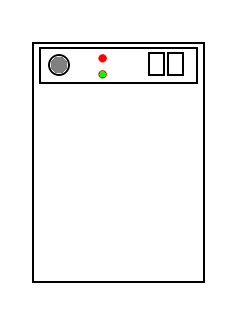
\includegraphics[scale=0.4]{figures/pictures/dishwasher.png}
%\rule{0.9\linewidth}{0.75\linewidth}
%\caption{Dishwasher}
\label{fig:dishwasher}
\end{wrapfigure}

This can be seen in the following example: The two agents from before, Anne and Bill have to empty out the dishwasher. They each have a preference against doing this, since they both spend time (costs) to do this.
In this example you can see that each agent expects the other agent to act, therefore no agent will act.

The formalization of this example would be: Consider the following planning task $\Pi = \langle s_0, A, \omega, \gamma \rangle $ with $s_0= fullDishwasher$, $\mathcal{A} = \{1,2\}$,
\\$A=\{emptyDishwasher_1, emptyDishwasher_2\}$ where \\
  $emptyDishwasher_1=\langle fullDishwasher, \neg fullDishwasher \rangle$, \\
   $\omega(emptyDishwasher_1)=1$, \\
   $emptyDishwasher_2= \langle fullDishwasher, \neg fullDishwasher \rangle$ and \\
 $\omega(emptyDishwasher_2)=2$. The goal formula is $\gamma = \neg fullDishwasher$.\\
The individual goal policies in this example are: $\pi_1=(s_0,emptyDishwasher_2, \gamma)$ and $\pi_2=(s_0, emptyDishwasher_1, \gamma)$ which means no agent will empty the dishwasher because every agent expects the other agent to empty the dishwasher.


Up to this point, the token has given the player that has it the right to perform an action, a right that none of the other players have. But tokens could also force a player to perform an action.

Consider the definition from before with some changes marked in color: \\
Given a regular planning task $\Pi = \langle s_0, A, \omega, \gamma \rangle $, the function \textit{tokenize-force} will transform the regular planning task into a tokenized planning task so that for all $a \in A$: \\
 if $a = \langle pre, \textit{eff} \rangle$, then
   $tokenize-force(a) =\langle pre \wedge hasToken^{\omega(a)}, \textit{eff } {\color{UniRed} \wedge doneAction^{\omega(a)}})$ \\
Former we define an Action
    $ giveToken^{ij} = \langle hasToken^i {\color{UniRed}\wedge doneAction^i}, \neg hasToken^i \wedge hasToken^j {\color{UniRed} \wedge \neg doneAction^i} \rangle $
    for all $i,j \in \mathcal{A}$
    \\
Then $ A^{Token}=\{tokenize(a)|a \in A\} \cup \{giveToken^{ij}|i,j \in \mathcal{A}, i \not = j\}
$ \\
Moreover: $\omega^{Token}(tokenize-force(a))= \omega(a)$ for all $a \in A$,
and $\omega^{Token}(giveToken^{ij}) = i$ for all $i,j \in \mathcal{A}$. \\
$s_0^{Token} = s_0 \cup \{\neg hasToken^i|i \in \mathcal{A} \backslash j\} \cup hasToken^j {\color{UniRed} \cup  \{ \neg doneAction^i| i \in \mathcal{A} \}}$ with $j \in \mathcal{A}, |j|=1$\\
With $j$ depending on the way the token should be introduced to the token:
\begin{enumerate}
  \item Table Token:
    The first agent to take the token off the table.
  \item give Token:
    a specified agent to be determined by the game maker
  \item random Token:
    a random agent
\end{enumerate}
Then $ \Pi^{\text{Token}} = \langle s_0^{Token}, A ^{\text{Token}}, \omega ^{\text{Token}}, \gamma \rangle $

In this case, the giveToken action has to cost something, otherwise the agents would just give each other the token back and forth

The changes imply that each agent can only pass on the token when that agent has performed an action.

This new token version also solves the infinite execution problem.

\begin{theorem}
  Under the condition of optimal plans one can prevent the appearance of infinite executions in solvable games with asynchronous execution order with the introduction of a force token based execution order.
\end{theorem}

\begin{proof}[proof sketch]
  The game is finished when the agent that has the token reaches a goal state. When an agent that has a plan gets handed the token, that player first has to perform an action, thereby lowering the subjective cost, and then that player has two possible actions:
  \begin{enumerate}
    \item keep the token and execute another action, which will lower the subjective costs of the remaining policy profile or
    \item give the token to the next player. in order to pass on the token the player that has found the plan would have already performed a perspective shift for the next player, in order to check if the next player could also find that plan and calculated the subjective cost of the remaining plan. The player that receives the token will always execute that plan or find a better plan and execute the better. plan.
  \end{enumerate}
  Every agent that will get the token in the plan will decrease the subjective cost of the policy profile, and because every agent decreases the subjective cost, the game is executable in infinite executions.
\end{proof}

\begin{theorem}
Under the condition of optimal plans one can prevent the appearance of deadlocks in solvable games with asynchronous execution order with the introduction of a force token based execution order with the exception of the table token introduction of the token.
\end{theorem}

\begin{proof}[proof sketch]
  Before any player can give away the token, that player has to perform an action. If a player that has found a plan gets the token, that agent first has to do an action. This contradicts the definition of a deadlock.
\end{proof}

The table token introduction of the token does not prevent deadlocks because in this case, no agent would take the token off the table, which causes a deadlock.

\begin{theorem}
  Under the condition of optimal plans one can prevent the appearance of deadlocks in solvable games with asynchronous execution order with the introduction of a token based execution order with the exception of the table token introduction of the token, as long as the giveToken action costs at least 1.
\end{theorem}

\begin{proof}[proof sketch]
  In order to have a policy profile with minimal costs, the agent will have to minimize the amount of giveToken actions in the policy profile. Therefore the agent will always perform an action themself instead of passing the token away, if possible. Because the agents have a common individual policy of keeping the subjective costs minimal, this contradicts the definition of a deadlock.
\end{proof}


A deadlock is different from a dead end. In a dead end, none of the agents' policies prescribe an action, not even for another agent. In the definition (2) above it becomes obvious that these are two different things. \todo{is this really needed? It looks unmotivated}
